\documentclass[10pt,a4paper]{article}
\usepackage[hmargin={30mm,30mm}, vmargin={25mm,25mm}]{geometry}
\usepackage{graphicx}
\usepackage{color}
\usepackage{eurosym}
\usepackage{fancyvrb}

\newenvironment{myitemize}
   {\begin{list}{$\bullet$}{
   \setlength{\parskip}{0mm}
   \setlength{\topsep}{3mm}
   \setlength{\partopsep}{0mm}
   \setlength{\itemsep}{4mm}
   \setlength{\rightmargin}{0mm}
   \setlength{\listparindent}{0mm}
   \setlength{\itemindent}{0mm}
   \setlength{\labelwidth}{2mm}
   \setlength{\parsep}{0mm}
   \setlength{\partopsep}{0mm}
   \setlength{\labelsep}{2mm}
   \setlength{\leftmargin}{\labelwidth+\labelsep}
   \let\makelabel\mylabel}}{
   \end{list}}
\pagestyle{empty}
\parindent0mm
\parskip2mm
%%%%%%%%%%%%%%%%%%%%%%
\begin{document}%BEGIN
\definecolor{sfondo}{rgb}{.97,.97,.9} 

%\pagecolor{sfondo}


\begin{center}
     \large\sf Torino, 9-11 February 2011 \ \par
      \Huge\sf Mini-school in Model Theory \ 

%%%%%%%%%%%%%%%%%%%%%%
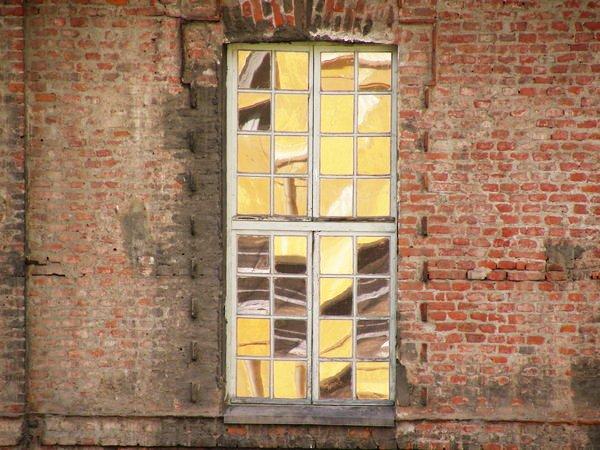
\includegraphics[width=110mm]{../Palazzo_Campana___Cortile2_by_dadexix86.jpg}%
\,\rotatebox{90}{\tiny\sf Foto: Davide Alberelli}

\large Aula S, Palazzo Campana, via Carlo Alberto 10

\end{center}

\vskip15mm
\begin{Verbatim}[fontfamily=helvetica]

Enrique Casanovas and Hans Adler will lecture about the basic theory of NIP.

Program 

Wednesday 9
  9:20 - 10:40  Enrique Casanovas: Tutorial
10:40 - 11:00  Coffee & croissants
11:00 - 12:20  Hans Adler: Tutorial
12:20 - 13:00  Elisabetta Pastori: Higher amalgamation problems: a group theoretical approach
13:00 - 14:20  Lunch
14:20 - 15:00  Krzysztof Krupinski: Algebraic properties of groups and rings in model theoretic contexts
15:00 - 15:40  Vincenzo Mantova: Zariski geometries through examples
 
Thursday 10
  9:20 - 10:40  Enrique Casanovas: Tutorial
10:40 - 11:00  Coffee & croissants
11:00 - 12:20  Hans Adler: Tutorial
12:20 - 13:00  Giuseppina Terzo: Exponential polynomials over an ACF
13:00 - 14:20  Lunch
14:20 - 15:00  Davide Penazzi: Reductions of elliptic curves and real closed valued fields
15:00 - 15:40  Jakub Gismatullin: Model theoretic connected components of linear groups
 
Friday 11
  9:20 - 10:40  Enrique Casanovas: Tutorial
10:40 - 11:00  Coffee & croissants
11:00 - 12:20  Hans Adler: Tutorial

\end{Verbatim}
\end{document}
